%----------------------------------------------------------------------------------------
%	PACKAGES AND OTHER DOCUMENT CONFIGURATIONS
%----------------------------------------------------------------------------------------
\documentclass[paper=a4, fontsize=11pt]{scrartcl} % A4 paper and 11pt font size
\usepackage[T1]{fontenc} % Use 8-bit encoding that has 256 glyphs
\usepackage{fourier} % Use the Adobe Utopia font for the document - comment this line to return to the LaTeX default
\usepackage[english]{babel} % English language/hyphenation
\usepackage{amsmath,amsfonts,amsthm} % Math packages
\usepackage{lipsum} % Used for inserting dummy 'Lorem ipsum' text into the template
\usepackage{sectsty} % Allows customizing section commands
\allsectionsfont{\centering \normalfont\scshape} % Make all sections centered, the default font and small caps
\usepackage{fancyhdr} % Custom headers and footers
\usepackage[]{mcode}
\usepackage{amsmath}
\usepackage{graphics}
\usepackage{graphicx}

\pagestyle{fancyplain} % Makes all pages in the document conform to the custom headers and footers
\fancyhead{} % No page header - if you want one, create it in the same way as the footers below
\fancyfoot[L]{} % Empty left footer
\fancyfoot[C]{} % Empty center footer
\fancyfoot[R]{\thepage} % Page numbering for right footer
\renewcommand{\headrulewidth}{0pt} % Remove header underlines
\renewcommand{\footrulewidth}{0pt} % Remove footer underlines
\setlength{\headheight}{13.6pt} % Customize the height of the header

\numberwithin{equation}{section} % Number equations within sections (i.e. 1.1, 1.2, 2.1, 2.2 instead of 1, 2, 3, 4)
\numberwithin{figure}{section} % Number figures within sections (i.e. 1.1, 1.2, 2.1, 2.2 instead of 1, 2, 3, 4)
\numberwithin{table}{section} % Number tables within sections (i.e. 1.1, 1.2, 2.1, 2.2 instead of 1, 2, 3, 4)

\setlength\parindent{0pt} % Removes all indentation from paragraphs - comment this line for an assignment with lots of text

%----------------------------------------------------------------------------------------
%	TITLE SECTION
%----------------------------------------------------------------------------------------

\newcommand{\horrule}[1]{\rule{\linewidth}{#1}} % Create horizontal rule command with 1 argument of height

\title{	
\normalfont \normalsize 
\horrule{0.5pt} \\[0.4cm] % Thin top horizontal rule
\huge ECE 532 HW 3: Subspaces \& Orthogonality\\ % The assignment title
\horrule{2pt} \\[0.5cm] % Thick bottom horizontal rule
}

\author{Qihong Lu} % Your name
\date{\normalsize\today} % Today's date or a custom date

\begin{document}

\maketitle % Print the title

%----------------------------------------------------------------------------------------
%	PROBLEM 1
%----------------------------------------------------------------------------------------

\section*{Question1 - Orthogonal Columns}
\textbf{Consider the matrix and vector}

$$
A = 
\begin{bmatrix}
3 & 1 \\
0 & 3 \\
0 & 4 
\end{bmatrix},
\;\;\;
b = 
\begin{bmatrix}
1 \\
3 \\
1 
\end{bmatrix}
$$
\textbf{a) By hand, find two orthonormal vectors that span the plane spanned by columns of A.}\\

By normalizing the first column, and substract the first column from the second. After that, I just need to normalize the second column. Then we can transform A to an orthogonal matrix: 
$$
A = 
\begin{bmatrix}
3 & 1 \\
0 & 3 \\
0 & 4 
\end{bmatrix}
\rightarrow
\begin{bmatrix}
1 & 1 \\
0 & 3 \\
0 & 4 
\end{bmatrix}
\rightarrow
\begin{bmatrix}
1 & 0 \\
0 & 3 \\
0 & 4 
\end{bmatrix}
\rightarrow
\begin{bmatrix}
1 & 0 \\
0 & 3/5 \\
0 & 4/5 
\end{bmatrix}
$$

Let's denoted it by Q:
$$
Q
=
\begin{bmatrix}
1 & 0 \\
0 & 3/5 \\
0 & 4/5 
\end{bmatrix}
$$
Now, the columns of Q are two orthonormal vectors that span the plane spanned by original columns of A. This can be seen easily because the original columns of A can be written as linear combinations of columns of Q, In particular: 

$$
a_{\bullet 1} = 
\begin{bmatrix}
3	\\
0	\\
0
\end{bmatrix}
= 3 q_{\bullet 1},
\;\;\;\;\;
a_{\bullet 2} = 
\begin{bmatrix}
1	\\
3	\\
4
\end{bmatrix}
= q_{\bullet 1} + 5 q_{\bullet 2}
$$\\\\

\textbf{b) Make a sketch of these vectors and the columns of A in three dimensions.}\\

\begin{center}
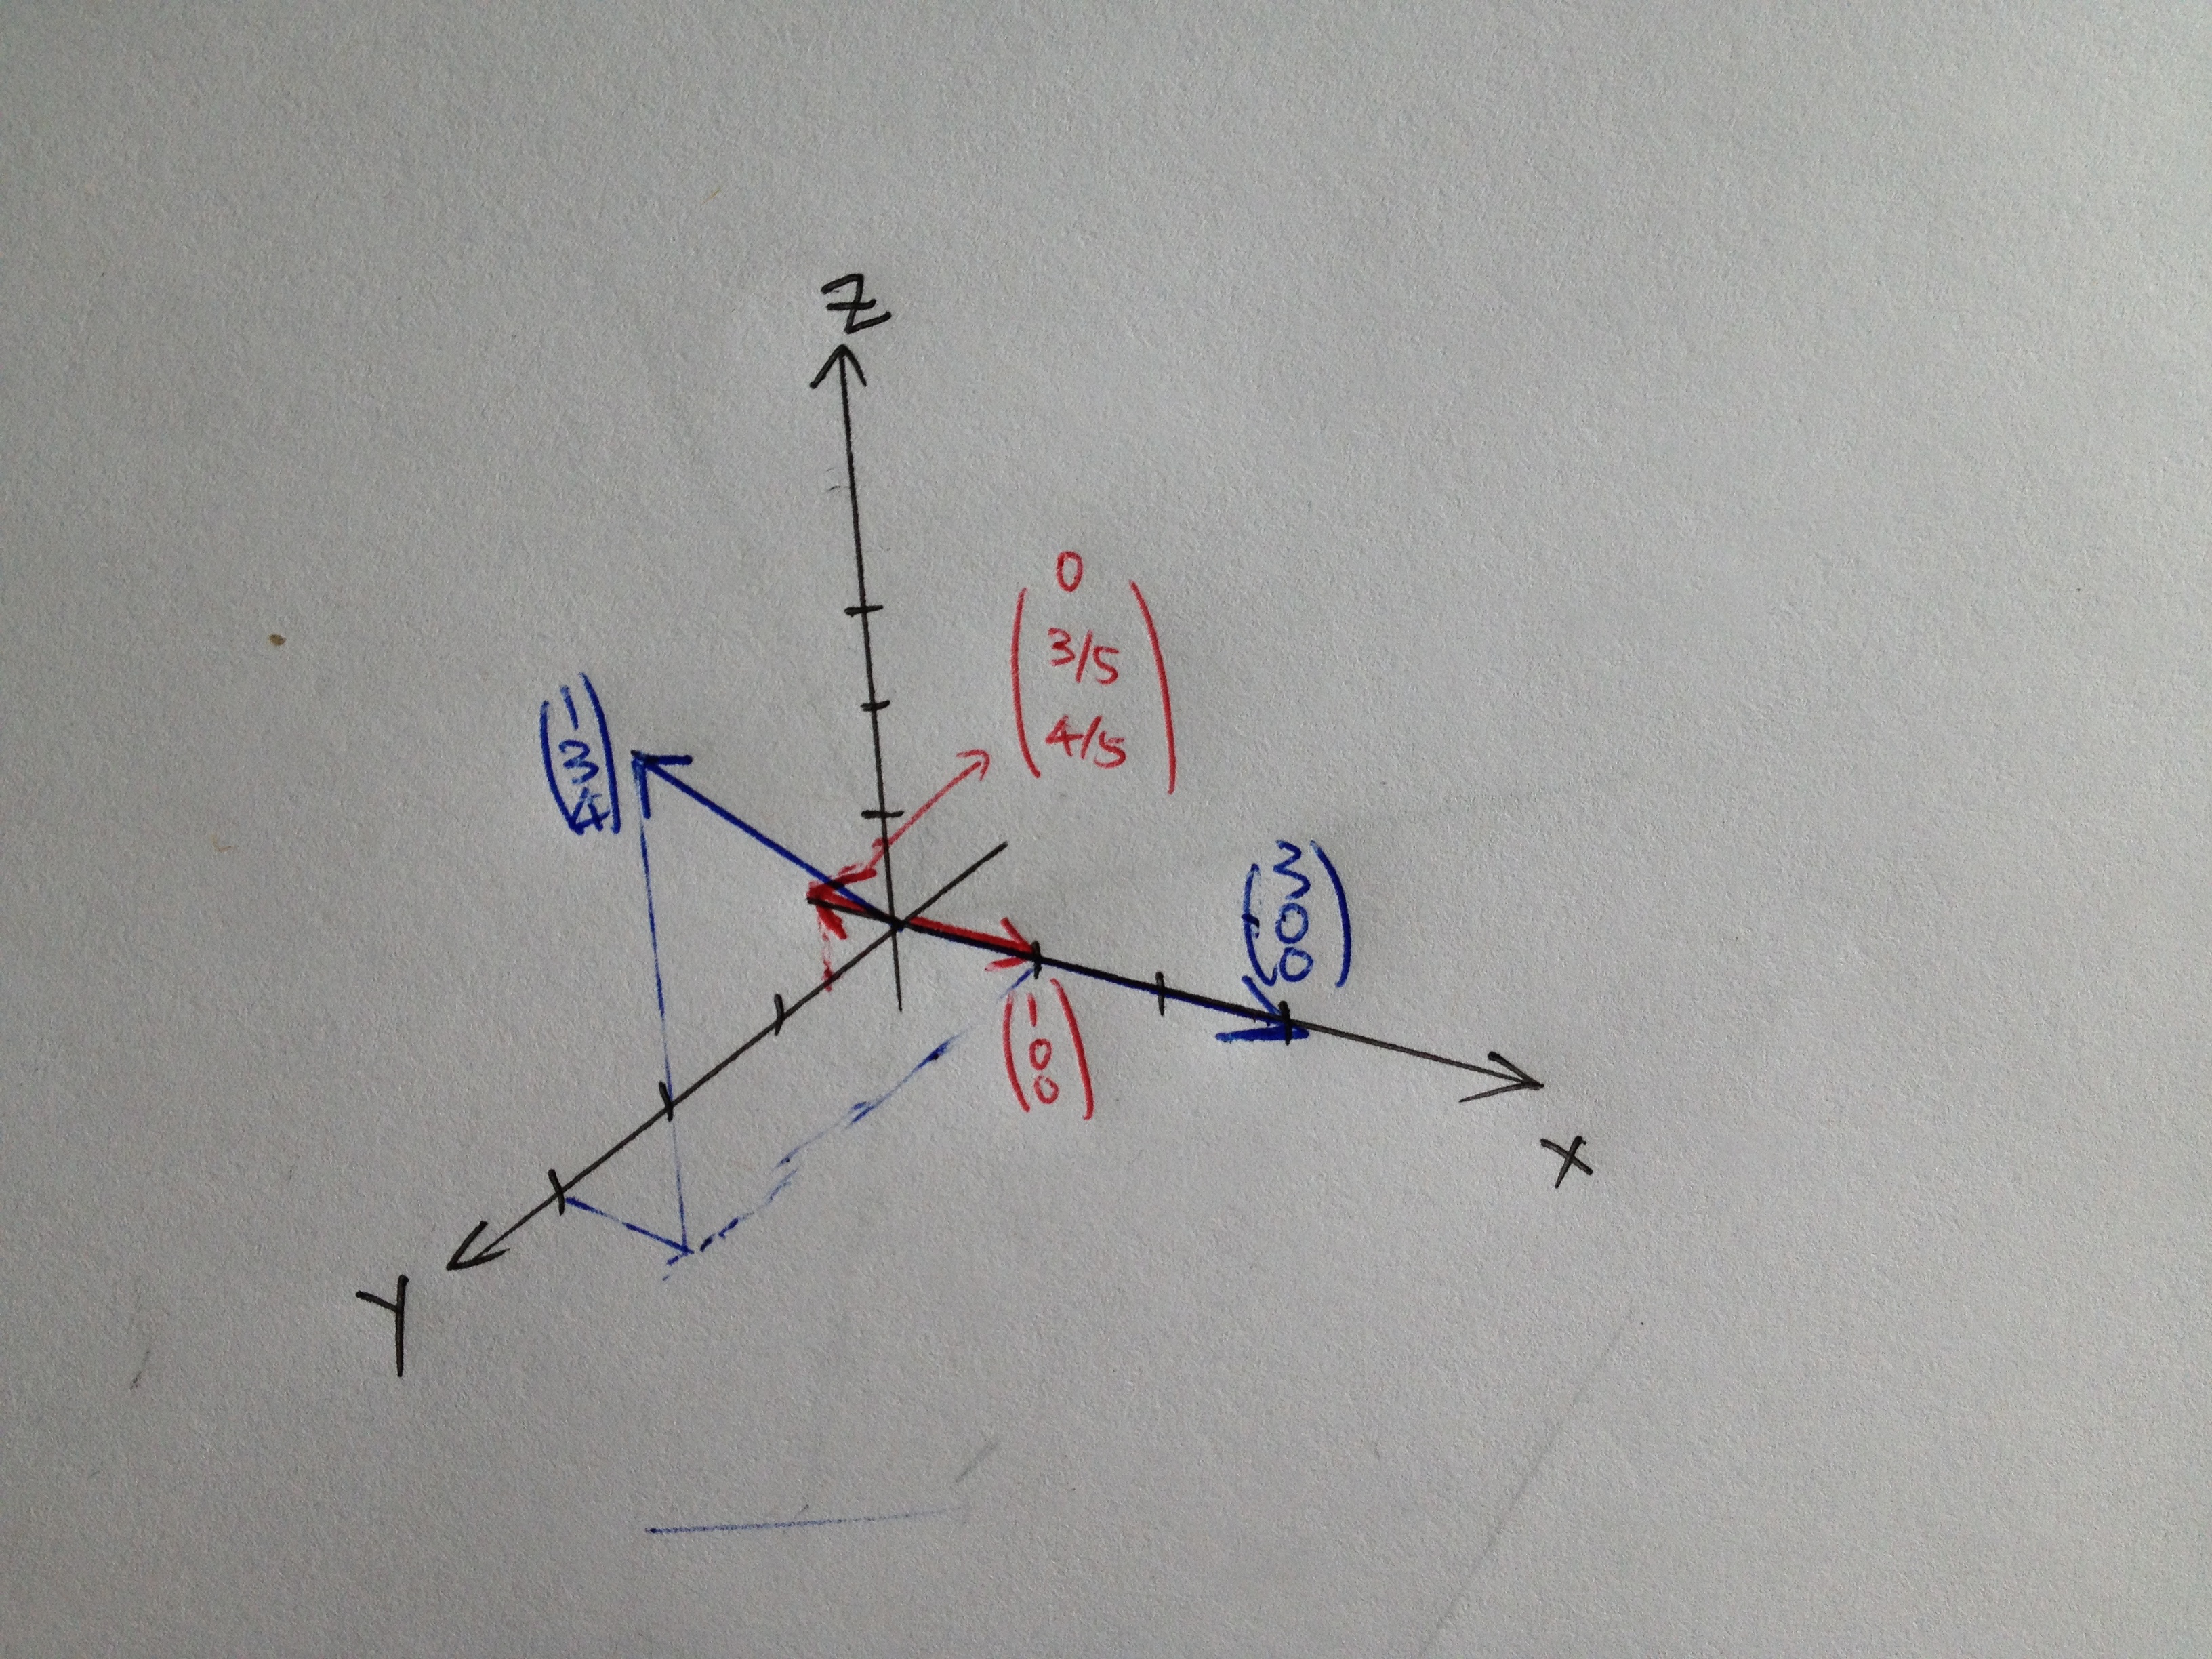
\includegraphics[scale=0.1]{sketch.JPG}\\
\end{center}

\textbf{c) Use these vectors to compute the LS estimate $\hat{b} = A(A^{T} A)^{-1} A^{T} b$.}\\ 

One can verify that $QQ^{T} b$ would give us the $\hat{b}$: 

$$
\hat{b} = 
QQ^{T} b = 
\begin{bmatrix}
1 & 0 \\
0 & 3/5 \\
0 & 4/5 
\end{bmatrix}
\;
\begin{bmatrix}
1 & 0  & 0\\
0 & 3/5  & 4/5 
\end{bmatrix}
\;
\begin{bmatrix}
1 \\
3 \\
1 
\end{bmatrix}
= 
\begin{bmatrix}
    1.0000	\\
    1.5600	\\
    2.0800
\end{bmatrix}
=
\hat{b} = A(A^{T} A)^{-1} A^{T} b
$$

Here's the MATLAB code that verify my computation:
\begin{lstlisting}
%% hw3-1-ece532
clear all; 
A = [3 0 0; 1 3 4]';
b = [1 3 1]';
% Q is an Orthogonal matrix that I came up for A 
Q = [1 0 0; 0 3/5 4/5]';
% compute beta in two ways
beta_1 = A * inv(A' * A) * A' * b;
beta_2 = Q * Q' * b;
% check if they are the same
all(beta_1 == beta_2)
\end{lstlisting}

\newpage
%----------------------------------------------------------------------------------------
%	PROBLEM 2
%----------------------------------------------------------------------------------------

\section*{Question2 - Tikhonov regularization}


\textbf{a) Solve the optimization problem }
$$
min \|b - Ax\|^{2} + \lambda \|x\|^{2}
$$
\textbf{by finding an expression for the minimizer $\hat{x}$.}\\

To solve for the minimizer, I want to take it's derivative and set it to zero. \\
First of all, take the derivative and do some simplifications: 
\begin{equation*} 
\begin{split}
\frac{d}{dx} [\|b - Ax\|^{2} + \lambda \|x\|^{2} ]
& =  \frac{d}{dx} [(b - Ax)^T(b - Ax) + \lambda x^Tx] \\
& =  \frac{d}{dx} [b^Tb - b^TAx - (Ax)^Tb + (Ax)^T(Ax) + \lambda x^Tx] \\
& =  0 - (b^TA)^T - (A^Tb)^T + 2A^TAx + 2\lambda x \\
& =  -2A^Tb + 2A^TAx + 2\lambda x
\end{split}
\end{equation*}

By setting the derivative to zero, we obtain the following: 
\begin{align*} 
-2A^Tb + 2A^TAx + 2\lambda x &= 0  \\ 
-A^Tb + A^TAx + \lambda x &= 0  	\\ 
(A^TA + \lambda I) x &= A^Tb 		\\
 x &= (A^TA + \lambda I)^{-1} A^Tb 	
\end{align*}


Therefore, the minimizer is $x= (A^TA + \lambda I)^{-1} A^Tb $\\


\textbf{b) Suppose that $A \in \mathbb{R}^{mxn}$, with $m < n$. Is there a unique solution to $L_2$ regularized least squares? Explain your answers.}\\

For the least square case, there will be infinitely many solutions. Because $m<n$, $rank(A) = rank (A^TA)$is at most $m$, and $A^TA$ is a nxn matrix. Therefore $(A^TA)$ is not invertible. \\

For equation (1), there is a unique solution if $(A^TA + \lambda I)$ is invertible. So I want to discuss its invertibility. \\
First of all, $\lambda I$ is a nxn matrix and it is certianly full rank. On the other hand, because $A \in \mathbb{R}^{mxn}$, so $A^TA \in \mathbb{R}^{nxn}$. Because $m < n$, so A cannot have more than m linearly independent vectors. So A is at most rank m. And $A^TA$ is also at most rank m. \\
Additionally, both $\lambda I$ and $A^TA$ are positive semidefinite. Because both of them are positive semidefnite and $\lambda I$ is full rank, their sum is going to be at least rank n, which means it is going to be full rank. \\
This is confirmed by my simulation. I genearted some random matrix A and found that $(A^TA + \lambda I)$ is always full rank. In this case, there will be a unique solution. \\



\newpage
%----------------------------------------------------------------------------------------
%	PROBLEM 3
%----------------------------------------------------------------------------------------

\section*{Question3 - Gram-Schmidt process}
\textbf{Write your own code to perform Gram-Schmidt orthogonalization. Your code should take as input a matrix $A \in \mathbb{R}^{mxn}$ and return as output a matrix $U \in \mathbb{R}^{mxr}$ where $U$ is orthogonal and has the same range as $A$.}\\
\textbf{a) Test your code by applying it to Problem 1 above.}\\

\begin{lstlisting}
%% a) apply my gram-schimit to problem 1 
A = [3 0 0; 1 3 4]';
b = [1 3 1]';
% compute weights using the normal equation
beta_1 = A * inv(A' * A) * A' * b;
% compute the weights using my gramSchmidit 
Q = gramSchmidtProcess(A);
beta_2 = Q * Q' * b;
% One can verify that beta1 and beta2 are the same 
\end{lstlisting}

\textbf{b) Use your code to determine the rank of the following matrices and compare the result to Matlab’s rank function}\\
$$
A_1 = 
\begin{bmatrix}
3 & 1 & 2 \\
0 & 3 & 3 \\
0 & 4 & 4 \\
6 & 1 & 4 
\end{bmatrix}
\;\;\;\;\;\;
A_2 = 
\begin{bmatrix}
1 & 1 & 2 \\
0 & 3 & 3 \\
0 & 4 & 4 \\
3 & 1 & 4 
\end{bmatrix}
$$

\begin{lstlisting}
%% b) Test my Gram-schimidt with the following matrices A1,A2
A1 = [3 0 0 6; 1 3 4 1; 2 3 4 4]';
A2 = [1 0 0 3; 1 3 4 1; 2 3 4 4]';
% orthogonalize them
Q1 = gramSchmidtProcess(A1)
Q2 = gramSchmidtProcess(A2)
% check ranks 
if (rank(A1) == size(Q1,2) && rank(A2) == size(Q2,2))
    disp('The ranks are correct');
end
\end{lstlisting}


\newpage
Here is the code I wrote for doing the Gram-Schmidt orthogonalization process: 

\begin{lstlisting}
%% Gram-Schmidt orthogonalization process
% Input: a matrix V
% Output: a orthogonal matrix Q, where span(col(Q)) == span(col(V))
function Q = gramSchmidtProcess(V)
% read dim and num vectors
dimension = size(V,1);
nCol = size(V,2);
%% if 1st column of A if the zero vector, just eliminate it
while V(:,1) == zeros(dimension,1)
    V = V(:,2:end);     % throw away zero column
    nCol = nCol-1;      % decrement numColumns 
end

%% start Gram-Schmidt process
% normalize the 1st column of A to get the 1st basis vector
Q(:,1) = V(:,1) / norm(V(:,1),2);
% orthogonalize the rest
for j = 2 : nCol
    % compute the projected component
    projection = zeros(dimension,1);
    for i = 1 : j-1
        projection = projection + Q(:,i)' * V(:,j) * Q(:,i);
    end
    % substract to get the orthogonal component
    temp = V(:,j) - projection;
    % if the orthogonal component is not zero vector
    if ~all(temp == 0)
        % normalize the orthogonal component to get the next column of Q
        Q(:,j) = temp / norm(temp);
    end
end
end

\end{lstlisting}
\newpage
%----------------------------------------------------------------------------------------
%	PROBLEM 4
%----------------------------------------------------------------------------------------

\section*{Question4 - Flower classification}
\textbf{a) Formulate the classification task as a least squares problem. Least squares will produce real-valued predictions, not discrete labels or categories. What might you do to address this issue?}\\
Answer: \\
In this problem, the things that we want to predict is the type of a given flower. I labeled three different type of flowers as discrete numerical values. In particular, 0 stands for setosa, 1 stands for versicolor and 2 stands for virginica. \\
After fitting the least square solution, the output value will be a real number. Namely, it is not going to be exactly 0 or 1 or 2. However, I can simply round it. Additionally, after rounding, if the output is smaller than zero, I just consider it as a 0; if the output is bigger than 2, I just consider it as a 2. (Empirically, I found most rounded outputs belong to the set $\{0, 1, 2\}$)\\


\textbf{b) Train a classifier using LS based on 40 labeled examples of each of the three flower types, and then test the performance of your classifier using the remaining 10 examples from each type. Repeat this with many different randomly chosen subsets of training and test. What is the average test error}\\
Answer: \\
The error is about $0.038000$\\


\textbf{c) Make a plot of average test error as a function of training set size.}

Answer: Here's the plot showing the average test set accuracy against the training set size: 
\begin{center}
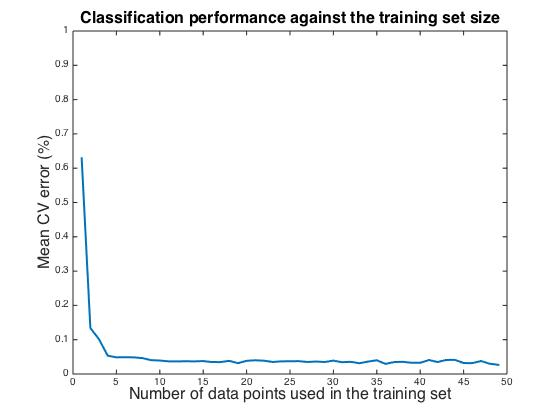
\includegraphics[scale=.5]{error_trainSize.jpg}
\end{center}

\newpage
\textbf{d) Now design a classifier using only the first three measurements (sepal length, sepal width, and petal length). What is the average test error in this case?}\\
Test set accuracy when using training set size of 40 is about $0.042000$.
Here's the plot showing the average test set accuracy against the training set size when using the first three features: 
\begin{center}
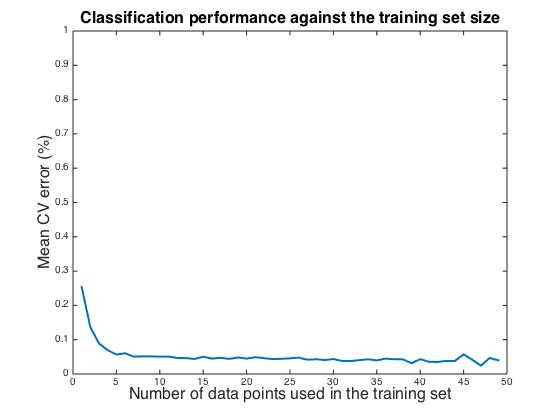
\includegraphics[scale=.5]{error_trainSize_3features.jpg}
\end{center}

\textbf{e) Use a 3d scatter plot to visualize the measurements in (d). Can you find a 2-dimensional subspace that the data approximately lie in? You can do this by rotating the plot and looking for plane that approximately contains the data points.}
\begin{center}
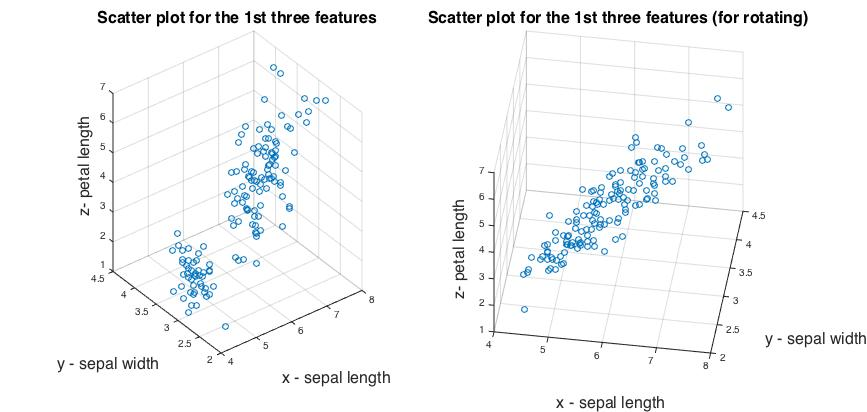
\includegraphics[scale=.45]{Xscatters.jpg}
\end{center}
After some rotation (the scatter plot on the right hand side), we can roughly see a plane that approximately contains all the data. 


\newpage
\textbf{f) Use this subspace to find a 2-dimensional classification rule. What is the average test error in this case?}

After doing the principle component analysis, I picked the first 2 column principle components as the basis for my 2D subspace. 
$$
v1 = 
\begin{bmatrix}
    0.3898   \\
   -0.0910   \\
    0.9164   
\end{bmatrix},
\;\;\;
v2 = 
\begin{bmatrix}
0.6392	\\
0.7431	\\
-0.1981
\end{bmatrix}
$$

By projecting the data points onto the space spanned by $v1$ and $v2$, we get the top plot. After some rotation (middle plot), we see that the data points lie in a 2D space. The plot on the button shows a visualization in that 2D space, where the coordinate systems are based on the two principle components $v1$ and $v2$. 
\begin{center}
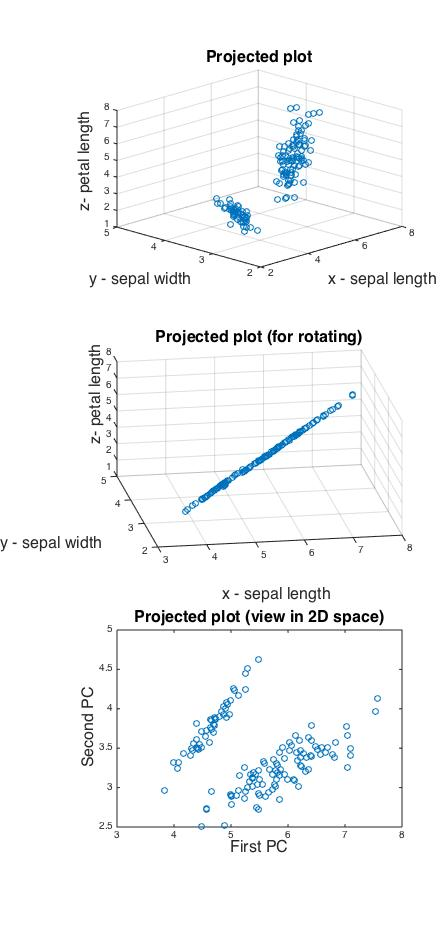
\includegraphics[scale=.46]{Xscatters_projected.jpg}
\end{center}

\newpage
Here's the error rate against the training size when I am classifying in 2D space, which is comparable to the performance when I use three features. 
\begin{center}
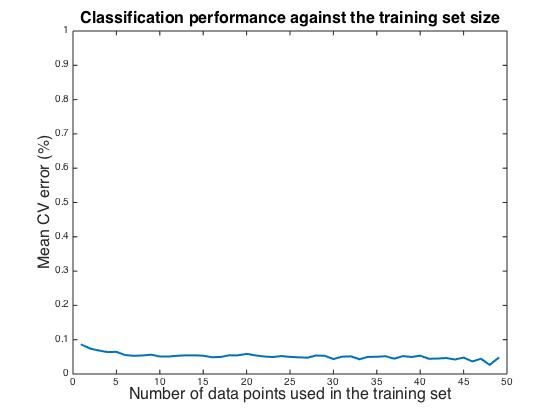
\includegraphics[scale=.5]{error_trainSize_2features.jpg}
\end{center}

\newpage
Here is the MATLAB code I wrote for question b to e. 
\begin{lstlisting}
%% ECE 532 - HW3 - Question 4
function classFlowers()
% initialization
clear all; clc
load fisheriris.mat
selectFirstThreeFeatures = 0;
projectOnTo2DSpace = 1; 
if projectOnTo2DSpace && ~selectFirstThreeFeatures
    warning('My projection code is based on the use of 3 features');
    selectFirstThreeFeatures = 1;
end

% some parameters
numData = 50;
% set the number of data points in the training data (< 50)
maxTrainSize = numData - 1;
% choose features (e.g. 1110 meas select the first three features)
if selectFirstThreeFeatures
    featureSelector = logical([1 1 1 0])
    % read the design matrix
    X = meas(:,featureSelector);
    if projectOnTo2DSpace
        % principle component analysis 
        pcs = pca(X);
        % use the subspace spanned by the 1st two PCs
        disp('Here are the basis for the lower dimensional subspace, where the data were projected')
        S = pcs(:,1:2)
        % calculate the projection matrix 
        projMat = S*inv(S'*S)*S';
        % do orthogonal projection 
        projectedX = X * projMat;
        X = projectedX(:,1:2);
    end
else
    % no feature selection & no projection
    X = meas;
end
% 0 = setosa
% 1 = versicolor
% 2 = virginica
y = [zeros(numData,1); ones(numData,1); 2*ones(numData,1)];

%% Run the analysis
% conduct multiple tests
numTrials = 50;
accuracy = nan(numTrials,maxTrainSize);
for trainSize = 1: maxTrainSize;
    for i = 1 : numTrials
        %% create vectors that randomly select training data
        holdOutIdx = getTrainingSetIndex(numData,trainSize);
        
        %% split the data into training and testing set
        Xtrain = X(holdOutIdx,:);
        ytrain = y(holdOutIdx);
        Xtest  = X(~holdOutIdx,:);
        ytest  = y(~holdOutIdx);
        
        %% fit the LS model
        beta = inv(Xtrain' * Xtrain) * Xtrain' * ytrain;
        
        %% compute the accuracy
        predictions = round(Xtest * beta);
        predictions = transformPredictions(predictions, y);
        accuracy(i,trainSize) = sum(predictions == ytest) / length(ytest);
    end
    
end
% compute the error
error = 1 - accuracy;
fprintf('Test set accuracy when using training set size of 40 is %f \n', mean(error(:,40)));

%% plot the performance 
plotPerformance_trainSize(error)

% plot the first three features in the scatter plot if we only use the 1st
% three features
if selectFirstThreeFeatures
    disp('Press something to see the scatter plots!'); pause;
    threeFeatureScatterPlots(meas)
    % if also project onto 2D space, plot the projected 2D scatter plot 
    if projectOnTo2DSpace
        disp('Press something to see the projected plots!'); pause;
        projectedScatterPlots(projectedX,X)
    end
end

end

%%%%%%%%%%%%%%%%%%%%%%%%%%%%%%%%%%%%%%%%%%%%%%%%%%%%%%%%%%%%%%%%%%%%%%%%%%%
%%%%%%%%%%%%%%%%%%%%%%%%%% Helper functions %%%%%%%%%%%%%%%%%%%%%%%%%%%%%%%
%%%%%%%%%%%%%%%%%%%%%%%%%%%%%%%%%%%%%%%%%%%%%%%%%%%%%%%%%%%%%%%%%%%%%%%%%%%

%% create vectors that randomly select the holdout set of given size
function holdOutIdx = getTrainingSetIndex(numData,trainSize)
% check input
if trainSize < 1
    error('Training size should be at least 1');
elseif trainSize >= numData
    error('Training size should be smaller than numData');
end
% preallocate
trainIdx.set = false(numData, 1);
trainIdx.ver = false(numData, 1);
trainIdx.vir = false(numData, 1);
% randomly choose some of them
trainIdx.set(randperm(numData, trainSize)) = true;
trainIdx.ver(randperm(numData, trainSize)) = true;
trainIdx.vir(randperm(numData, trainSize)) = true;
% concatenate the index vector
holdOutIdx = [trainIdx.set; trainIdx.ver; trainIdx.vir];
end


%% handle impossible predictions
% the range of y is {0, 1, 2}, so if the classifer under/over shot, force
% it to be the closest label in the range
function predictions = transformPredictions(predictions, y)
% this is written in a more genearl form that is not specific to {0,1,2}
% range
ymax = max(y);
ymin = min(y);
predictions(predictions > ymax) = ymax;
predictions(predictions < ymin) = ymin;
end


%% Plot the performance against trainSize
function plotPerformance_trainSize(error)
FS = 16;
% plot the error vector, which records the error by training set size
plot(mean(error),'LineWidth',2)
% add some descriptions
ylim([0,1])
title('Classification performance against the training set size', 'fontsize', FS)
xlabel('Number of data points used in the training set', 'fontsize', FS)
ylabel('Mean CV error (%)', 'fontsize', FS)
end

%% create 3 d scatter plots for 3 features
function threeFeatureScatterPlots(meas)
FS = 16;

% create the scatter plots
subplot(1,2,1)
scatter3(meas(:,1),meas(:,2),meas(:,3))
title('Scatter plot for the 1st three features', 'fontsize', FS)
xlabel('x - sepal length', 'fontsize', FS)
ylabel('y - sepal width', 'fontsize', FS)
zlabel('z- petal length', 'fontsize', FS)

% create the SAME scatter plots (for rotating)
subplot(1,2,2)
scatter3(meas(:,1),meas(:,2),meas(:,3))
title('Scatter plot for the 1st three features (for rotating)', 'fontsize', FS)
xlabel('x - sepal length', 'fontsize', FS)
ylabel('y - sepal width', 'fontsize', FS)
zlabel('z- petal length', 'fontsize', FS)

end

%% plot the projected 2D scatter plot 
function projectedScatterPlots(projectedX,X)
FS = 16;
% create the PROJECTED scatter plots
subplot(3,1,1)
scatter3(projectedX(:,1),projectedX(:,2),projectedX(:,3))
title('Projected plot', 'fontsize', FS)
xlabel('x - sepal length', 'fontsize', FS)
ylabel('y - sepal width', 'fontsize', FS)
zlabel('z- petal length', 'fontsize', FS)

% create the PROJECTED scatter plots
subplot(3,1,2)
scatter3(projectedX(:,1),projectedX(:,2),projectedX(:,3))
title('Projected plot (for rotating)', 'fontsize', FS)
xlabel('x - sepal length', 'fontsize', FS)
ylabel('y - sepal width', 'fontsize', FS)
zlabel('z- petal length', 'fontsize', FS)

% create the PROJECTED scatter plots (for rotating)
subplot(3,1,3)
plot (X(:,1), X(:,2),'o');
title('Projected plot (view in 2D space)', 'fontsize', FS)
xlabel('First PC', 'fontsize', FS)
ylabel('Second PC', 'fontsize', FS)

end

\end{lstlisting}

\end{document}